% 图 2.4 单位球上 theta 与 theta+dtheta 之间的环带（面积 2*pi*sin(theta)*dtheta）
\documentclass[tikz,border=5pt]{standalone}
\usetikzlibrary{arrows.meta}
\usepackage{amsmath}
\usepackage{bm}
\usepackage{fontspec}
\setmainfont{Times New Roman}
\begin{document}
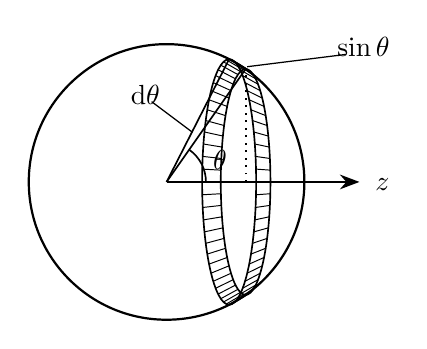
\begin{tikzpicture}[line width=0.8pt,>=Stealth]
\def\R{1.75}
\def\thA{55}   % theta
\def\dth{8}    % dtheta
% 球轮廓
\draw (0,0) circle (\R);
% 环带两条小圆（投影椭圆）：中心 (R cos, 0)，y 半径 R sin，x 半径 0.22*R sin
\pgfmathsetmacro{\cA}{\R*cos(\thA)}
\pgfmathsetmacro{\rA}{\R*sin(\thA)}
\pgfmathsetmacro{\cB}{\R*cos(\thA+\dth)}
\pgfmathsetmacro{\rB}{\R*sin(\thA+\dth)}
\def\kx{0.22}
% 环带阴影：两椭圆对应点连线
\foreach \deg in {0,6,...,354}{
  \pgfmathsetmacro{\xa}{\cA+\kx*\rA*cos(\deg)}
  \pgfmathsetmacro{\ya}{\rA*sin(\deg)}
  \pgfmathsetmacro{\xb}{\cB+\kx*\rB*cos(\deg)}
  \pgfmathsetmacro{\yb}{\rB*sin(\deg)}
  \draw[line width=0.35pt] (\xa,\ya) -- (\xb,\yb);
}
\draw[line width=0.6pt] (\cA,0) ellipse ({\kx*\rA} and {\rA});
\draw[line width=0.6pt] (\cB,0) ellipse ({\kx*\rB} and {\rB});
% sin(theta) 虚线半径（椭圆内竖直线）
\draw[dotted,line width=0.7pt] (\cA,0) -- (\cA,\rA);
% 两条半径线与角度
\draw[line width=0.6pt] (0,0) -- (\cA,\rA);
\draw[line width=0.6pt] (0,0) -- (\cB,\rB);
\draw[line width=0.6pt] (0.5,0) arc[start angle=0,end angle=\thA,radius=0.5];
\node at (0.68,0.28) {$\theta$};
\node at (-0.27,1.10) {$\mathrm{d}\theta$};
\draw[line width=0.45pt] (-0.19,1.02) -- (0.33,0.63);
% z 轴
\draw[->,line width=0.9pt] (0,0) -- (2.45,0) node[below=1pt,right=2pt] {$z$};
% sin theta 标注
\node at (2.5,1.72) {$\sin\theta$};
\draw[line width=0.45pt] (2.28,1.62) -- (\cA+0.02,\rA+0.03);
\end{tikzpicture}
\end{document}
